\chapter{Upgrade of the Upstream Tracker}
\label{ref:ut}

Located in the fringing fields in front of the LHCb dipole Magnet,
the Upstream Tracker (UT) plays an important role in improving the tracking
quality and speeding up trigger decisions:
Combining hits from VELO, SciFi, and UT provides the best \pt resolution
and reduce the rate of random combinations from VELO and SciFi to form
ghost tracks to about one fourth.
Furthermore, combining hits from VELO and UT removes low-\pt tracks and narrows
down the hit search window in SciFi, allowing for a faster track reconstruction
which leads to faster trigger decisions.

The University of Maryland group is responsible for the design, testing, and
commissioning of the peripheral and power regulating electronics;
An overview of the UT, discussed in \cref{ref:ut:overview},
summarizes the specifications and utilities of these electronics,
together with the sensors.
The author is tasked to test and develop quality assurance procedure for
the Data Control Board (DCB),
part of the peripheral electronics,
which is responsible to concentrate sensor readout and to control the UT
detector;
more details on DCB is described in \cref{ref:ut:dcb}.
In doing so, the author gained understanding on the data acquisition and control
system of the UT.
These systems are described in \cref{ref:ut:daq} and \cref{ref:ut:ctrl},
respectively.


\section{Overview of the UT detector}
\label{ref:ut:overview}

The UT consists of 4 planar detection layers with full LHCb acceptance coverage.
As shown in \cref{fig:ut-layers},
the first and last layers are vertical,
whereas the second and third are rotated by a stereo angle of $\pm 5^\circ$
to form a $x$-$u$-$v$-$x$ configuration.
The vertical planes provide highest hit resolution in the bending plane
($x$-$y$);
the rotated planes provide a measurement in the non-bending direction ($z$).

\begin{figure}[!htb]
    \centering
    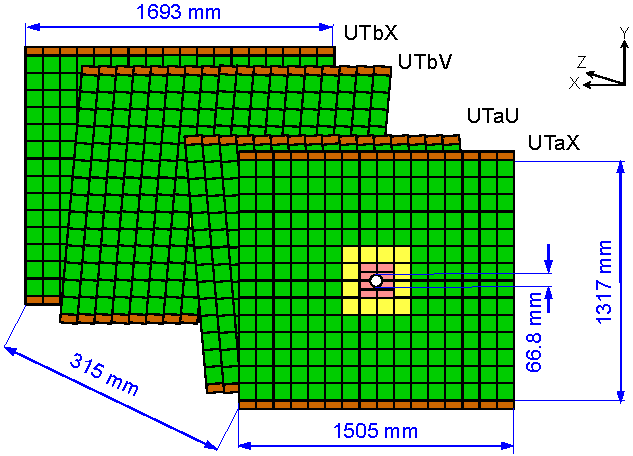
\includegraphics[width=0.7\textwidth]{./figs-lhcb-upgrade-overview/tracking/ut_upgrade.pdf}
    \caption{
        Four detection layers of UT,
        arranged in a $x$-$u$-$v$-$x$ configuration.
    }
    \label{fig:ut-layers}
\end{figure}

Each detection layer is made of a number of staves,
a vertical strip of sensors and their readout electronics;
the staves are discussed in \cref{ref:ut:overview:stave}.
The sensor readouts are collected by the electronics hosted inside Peripheral
Electronics (PEPI) crates at the top and bottom of the detection layer,
and are described in \cref{ref:ut:overview:pepi}.
To reduce radiation damage, the low voltage regulators (LVRs),
which supply power to the detector electronics,
are placed further away from the beam at the service bay;
a brief description of the LVR is given in \cref{ref:ut:overview:lvr}.


\subsection{Stave}
\label{ref:ut:overview:stave}


\subsection{PEPI}
\label{ref:ut:overview:pepi}


\subsection{LVR}
\label{ref:ut:overview:lvr}


\section{The Data Control Board (DCB)}
\label{ref:ut:dcb}


\section{Data acquisition in UT}
\label{ref:ut:daq}

\subsection{TELL40 the event builder}


\subsection{Data transmission path}


\section{Control system of UT}
\label{ref:ut:ctrl}


\subsection{Timing and Fast Control (TFC)}


\subsection{Slow control for detector initialization and monitoring}
